\section{Auswertung}
\label{sec:Auswertung}
Für die Temperatur wurde eine Messunsicherheit von $\symup{\Delta} T = \SI{0.2}{\kelvin}$ angenommen. Die Messunsicherheit der Zeit wird als
$\symup{\delta} t = \SI{0.1}{\second}$\footnote{Die Messunicherheit der Zeit wird mit dem kleinen $\symup{\delta}$ beschrieben, 
da das große $\symup{\Delta}$ für die Phasendifferenz gebraucht wird.} angesehen. Jegliche Fehlerrechnung wurde mit der Python Bibliothek 
uncertainties \cite{uncertainties} absolviert. Trotz dessen sind die Formeln für die Unsicherheiten am Ende der Auswertung angegeben. 
\subsection{Statisches Vefahren}  
\subsubsection{Vergleich der Temperaturverläufe}
\begin{figure}
  \label{stat2}
  \begin{subfigure}{0.48\textwidth}
    \centering
    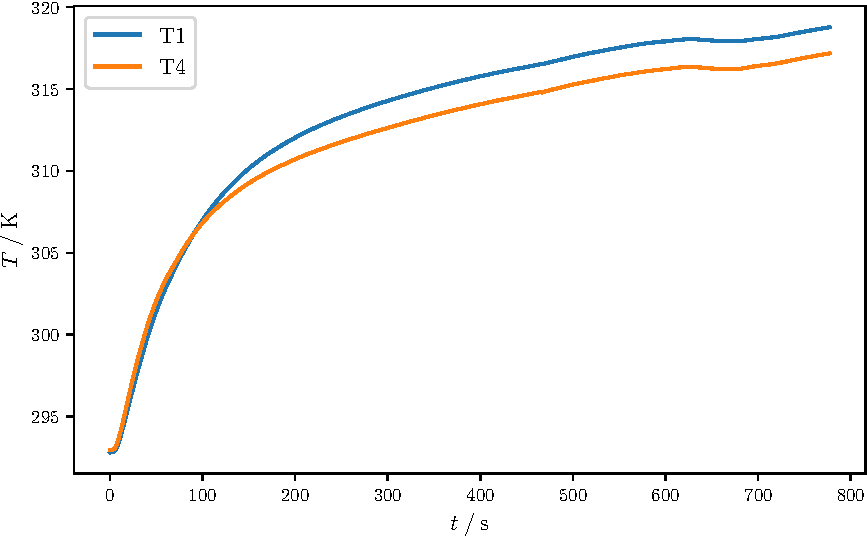
\includegraphics[width = \textwidth]{build/stat14.pdf}
    \caption{Temperaturverlauf $T_1$ und $T_4$}
    \label{fig:stat14}
  \end{subfigure}
  \begin{subfigure}{0.48\textwidth}
    \centering
    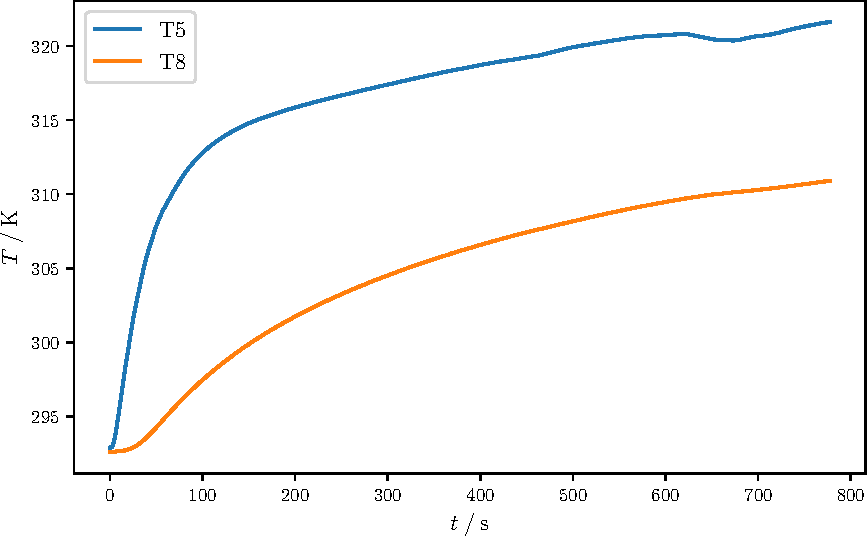
\includegraphics[width = \textwidth]{build/stat58.pdf}
    \caption{Temperaturverlauf $T_5$ und $T_8$}
    \label{fig:stat58}
  \end{subfigure}
\end{figure}
Bei dem Vergleichen der Kurven fällt auf, dass alle vier Kurven zu Beginn einen starken Temperaturanstieg repräsentieren, welcher jedoch schnell wieder abschwächt.
Dennoch verhalten sich die Temperaturen $T_1$ und $T_4$ anfangs beinahe identisch, wobei die Temperaturen $T_5$ und $T_8$ dort Diskrepanzen aufzeigen. $T_5$ steigt 
sehr stark an und flacht vergleichsweise schnell wieder ab, während die Temperatur $T_8$ eine eher verhaltene Steigung aufweist, denn diese steigt sehr langsam an, besitzt
im Gegenzug dazu keinen abrupten Steigungsverlust. Nach dem beinahe identischen Verhalten fällt die Kurve von $T_4$ früher ab, wonach dann eine kleine, annähernd konstante
Differenz zwischen den beiden Temperaturen herrscht. Aufgrund der verhaltenen Steigung der Temperaturkurve von $T_8$ ist die Differenz zwischen den beiden Kurven aus der 
Graphik \eqref{fig:stat58} schon von Anfang an sehr groß, wobei sich diese ab dem Zeitpunkt $t \approx \SI{150}{\second}$ eingestellt hat. Als letzte Gemeinsamkeit erkennt man leicht, dass
alle Kurven einen leichten Abfall bei $t \approx \SI{620}{\second}$ erleiden.
\subsubsection{Die beste Wärmeleitfähigkeit}
\begin{table}
  \centering
  \caption{Temperaturen nach $\SI{700}{\second}$}
  \label{tab:Waeremleitfaehigkeit}
  \sisetup{table-format = 3.2}
  \begin{tabular}{S S S S}
     \toprule
     {$T_1 \mathbin{/} \si{\kelvin}$} & {$T_4 \mathbin{/} \si{\kelvin}$} & {$T_5 \mathbin{/} \si{\kelvin}$} & {$T_8 \mathbin{/} \si{\kelvin}$}  \\
     \midrule
     318.06 & 316.42 & 320.66 & 310.28 \\
      \bottomrule
  \end{tabular}
\end{table}
Wie man anhand der Tabelle \eqref{tab:Waeremleitfaehigkeit} erkennen kann, hat Aluminium die beste Leitfähigkeit.
\subsubsection{Wärmestrom}
Für die Berechnung des Wärmestroms dient die Gleichung \eqref{eqn:Wärmemenge}. Jedoch lässt sich in diesem Fall die Wärmestromdichte
$j_w$ nicht mit dem Differntialquotient $\sfrac{\partial T}{\partial x}$ sondern nur mit dem Differenzenquotienten $\sfrac{\symup{\Delta}T}{\symup{\Delta} x}$
berechnen, so dass der Wärmestrom auch durch einen Differenzenquotienten dargestellt wird. 
Für den Abstand zwischen zwei Thermoelementen  wurde $\symup{\Delta} x = \SI{0.03}{\meter}$ gemessen.
\begin{table}
  \centering
  \caption{Errechnete Wärmeströme}
  \label{tab:Wärmestrom}
  \sisetup{table-format = 1.4}
  \begin{tabular}{S[table-format = 3.0] 
    S[table-format = 1.2] @{${}\pm{}$} S[table-format = 0.2] 
    S[table-format = 1.2] @{${}\pm{}$} S[table-format = 0.2] 
    S[table-format = 1.2] @{${}\pm{}$} S[table-format = 0.2] 
    S[table-format = 1.2] @{${}\pm{}$} S[table-format = 0.2]}
    \toprule
    {$t \mathbin{/} \si{\second}$} 
    & \multicolumn{2}{c}{$\frac{\symup{\Delta} Q_\text{Me}}    {\symup{\Delta}t} \mathbin{/} \si{\joule\second\tothe{-1}}$}
    & \multicolumn{2}{c}{$\frac{\symup{\Delta} Q_\text{Me,k}}  {\symup{\Delta}t} \mathbin{/} \si{\joule\second\tothe{-1}}$}  
    & \multicolumn{2}{c}{$\frac{\symup{\Delta} Q_\text{Al}}    {\symup{\Delta}t} \mathbin{/} \si{\joule\second\tothe{-1}}$}
    & \multicolumn{2}{c}{$\frac{\symup{\Delta} Q_\text{St}}    {\symup{\Delta}t} \mathbin{/} \si{\joule\second\tothe{-1}}$}\\
    \cmidrule(lr){2-3} \cmidrule(lr){4-5} \cmidrule(lr){6-7} \cmidrule(lr){8-9}
    \midrule
    100 & 7.49 & 0.38 & 4.65 & 0.22 & 7.51 & 0.76 & 3.57 & 0.07 \\
    200 & 5.18 & 0.38 & 3.43 & 0.22 & 5.08 & 0.76 & 3.10 & 0.07 \\
    300 & 4.63 & 0.38 & 3.16 & 0.22 & 4.66 & 0.76 & 2.82 & 0.07 \\
    500 & 4.63 & 0.38 & 3.15 & 0.22 & 4.78 & 0.76 & 2.61 & 0.07 \\
    700 & 4.28 & 0.38 & 2.92 & 0.22 & 4.44 & 0.76 & 2.35 & 0.07 \\
    \bottomrule
  \end{tabular}
\end{table}
Der Fehler lässt sich mittels der Fehlerfortpfllanzung nach Gauß berechnen:
\begin{equation}
  \symup{\Delta} \left ( \frac{\symup{\Delta}Q}{\symup{\Delta} t} \right) = \kappa A \frac{\symup{\Delta} T }{\SI{0.03}{\metre}}
\end{equation}
\subsubsection{Vergleich der Temperaturdiffernzen}
\begin{figure}
  \begin{subfigure}{0.48\textwidth}
    \centering
    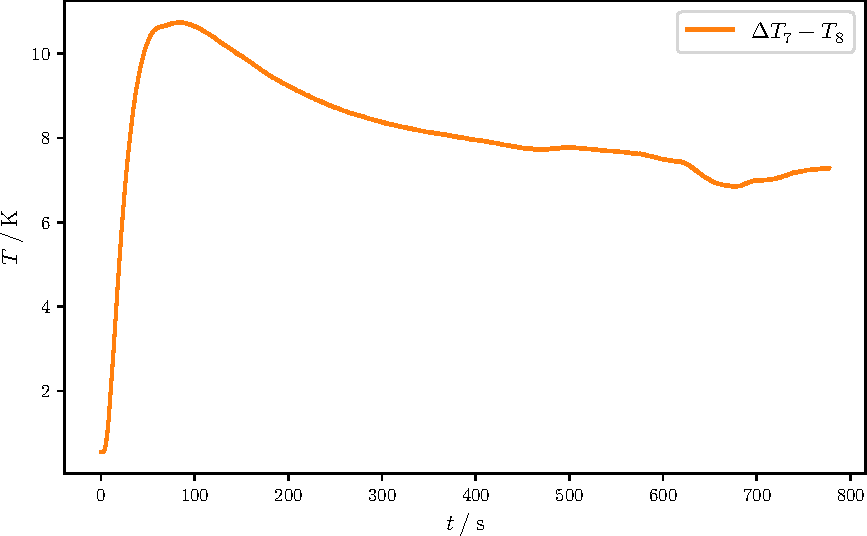
\includegraphics[width = \textwidth]{build/statDifSt.pdf}
    \caption{Temperaturdifferenz $\symup{\Delta}T_\text{St}$}
    \label{fig:statDifSt}
  \end{subfigure}
  \begin{subfigure}{0.48\textwidth}
    \centering
    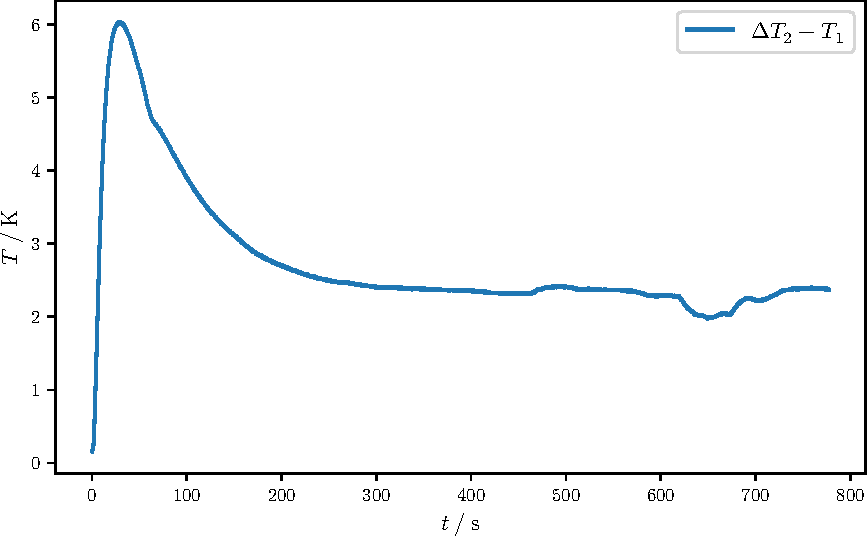
\includegraphics[width = \textwidth]{build/statDifMek.pdf}
    \caption{Temperaturdifferenz $\symup{\Delta}T_\text{Me}$}
    \label{fig:statDifMek}
  \end{subfigure}
\end{figure}
Bei der Betrachtung der Graphen \eqref{fig:statDifSt} und \eqref{fig:statDifMek} erkennt man instantan, dass bei beiden
Kurven ein Maximum kurz vor $t = \SI{100}{\second}$ erreicht wird, wobei beide danach 
wieder abfallen. Dies liegt der Ursache zu Grunde, dass die Temperaturen an den inneren und äußeren Thermoelementen im Bereich der Raumtemperatur liegen. 
Erwärmt man jedoch den Stab steigt die Temperatur am inneren  Thermoelement deutlich schneller an als die an dem äußeren Thermoelement, da die Wärme erstmal
in einer gewissen Zeit nach außen strömen muss, so dass ein zeitlicher Verzug entsteht. Bei näherer Betrachung wird die Stärke des Abfalls auffällig, da die
Temperaturdifferenz des Stahlstabes deutlich langsamer abfällt als die des großen Messingstabes. 
\subsection{Dynamisches Verfahren}
\begin{figure}
  \caption{Temperaturen des großen Messingstabs}
  \centering
  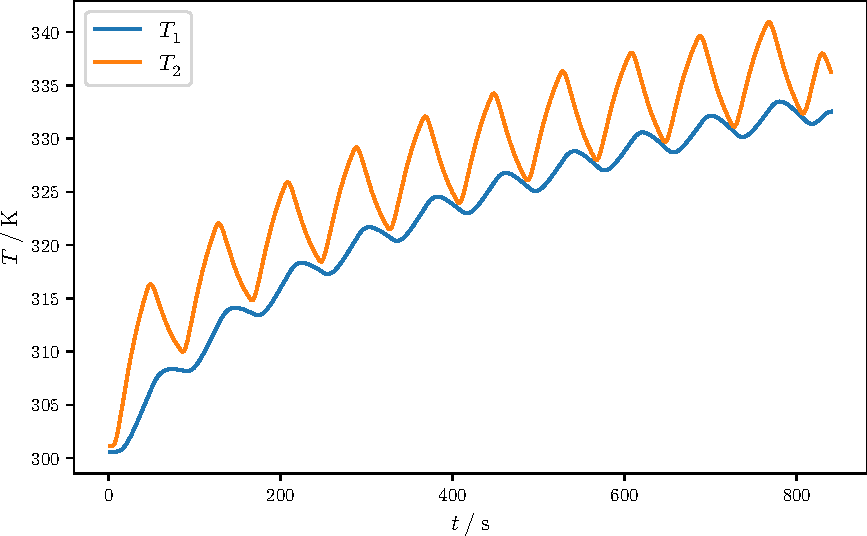
\includegraphics[width = \textwidth]{build/Me.pdf}
\end{figure}
\begin{table}
  \centering
  \label{tab:AmplitudeMessing}
  \caption{Amplituden und Phasendifferenzen des großen Messingstabs}
  \sisetup{table-format = 1.2}
  \begin{tabular}
    {S @{${}\pm{}$} S
     S @{${}\pm{}$} S
     S[table-format = 2.2] @{${}\pm{}$} S
     S[table-format = 3.4] @{${}\pm{}$} S[table-format = 2.4]}
     \toprule
     \multicolumn{2}{c}{$A_1 \mathbin{/} \si{\kelvin}$}       &
     \multicolumn{2}{c}{$A_2 \mathbin{/} \si{\kelvin}$}       &  
     \multicolumn{2}{c} {$\symup{\Delta}t_\text{Me}  \mathbin{/} \si{\second}$} &
     \multicolumn{2}{c}{$\kappa_\text{Me} \mathbin{/} \si{\watt\metre\tothe{-1}\kelvin\tothe{-1}}$}\\
     \cmidrule(lr){1-2} \cmidrule(lr){3-4} \cmidrule(lr){5-6} \cmidrule(lr){7-8}
     \midrule
     0.10 & 0.28 & 1.24 & 0.28 & 26.00 & 0.14 &  22.5495 & 25.1596\\
     0.35 & 0.28 & 2.11 & 0.28 & 20.00 & 0.14 &  41.0822 & 18.5464\\
     0.53 & 0.28 & 2.34 & 0.28 & 16.00 & 0.14 &  62.1238 & 22.6669\\
     0.65 & 0.28 & 2.49 & 0.28 & 16.00 & 0.14 &  68.6903 & 22.7777\\
     0.78 & 0.28 & 2.67 & 0.28 & 14.00 & 0.14 &  85.6819 & 26.0541\\
     0.85 & 0.28 & 2.66 & 0.28 & 14.00 & 0.14 &  92.4183 & 28.0298\\
     0.90 & 0.28 & 2.73 & 0.28 & 14.00 & 0.14 &  95.0154 & 28.0654\\
     0.94 & 0.28 & 2.74 & 0.28 & 14.00 & 0.14 &  98.5527 & 29.0265\\
     1.01 & 0.28 & 2.82 & 0.28 & 12.00 & 0.14 & 119.7985 & 34.3854\\
     1.04 & 0.28 & 2.85 & 0.28 & 12.00 & 0.14 & 122.0194 & 34.7186\\
      \bottomrule
  \end{tabular}
\end{table}
Mit dem gegebenen Literaturwert für Dichte von Messing $\rho_\text{Me} = \SI{8520}{\kilogram\per\meter\cubed}$, der gegebenen spezifischen Wärmekapazität 
$c_\text{Me} = \SI{385}{\joule\per\kilogram\per\kelvin}$ und dem gemessen Abstand $\symup{\Delta} x = \SI{0.03}{\meter}$ lässt sich der Mittelwert 
der Wärmeleitfähigkeit zu
\begin{equation}
\overline{\kappa}_\text{Me} = \SI{81(9)}{\watt\per\metre\per\kelvin}
\label{eqn:frequenz}
\end{equation}
berechnen. Die Periodendauer dieser Temperaturwelle beträgt $\tau = \SI{80.0(1)}{\second}$, so dass sich eine Frequenz von
\begin{equation}
  f = \SI{0.012500(16)}{\per\second}
\end{equation}
ergibt. Mit Hilfe der Gleichung \eqref{eqn:wellenlänge}
lässt sich die Wellenlänge zu 
\begin{equation}
  \lambda_\text{Me} = \SI{0.157(8)}{\metre}
\end{equation}
berechnen.
\begin{figure}
  \caption{Temperaturen des Aluminiumstabs}
  \centering
  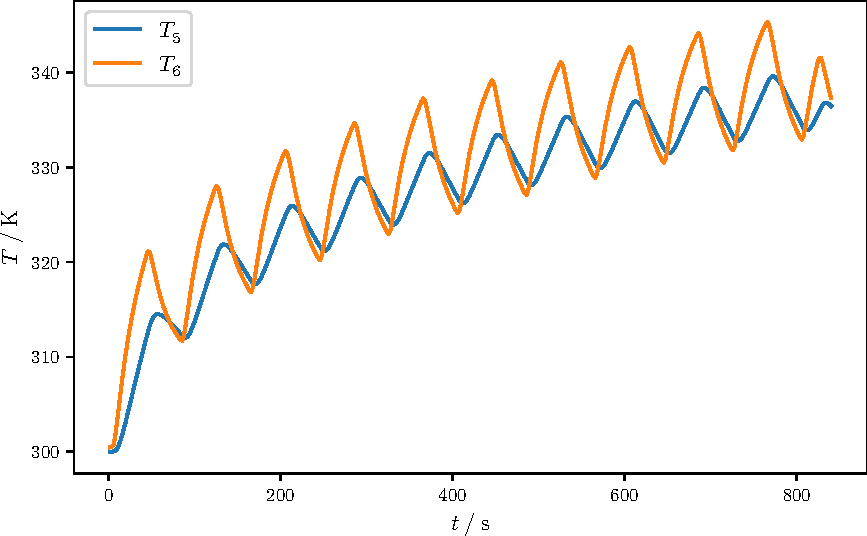
\includegraphics[width = \textwidth]{build/Al.pdf}
\end{figure}
\begin{table}
  \centering
  \label{tab:AmplitudeAluminium}
  \caption{Amplituden und Phasendifferenzen des Aluminiumstabs}
  \sisetup{table-format = 1.2}
  \begin{tabular}{
    S @{${}\pm{}$} S
    S @{${}\pm{}$} S
    S[table-format = 2.2] @{${}\pm{}$} S
    S[table-format = 3.4] @{${}\pm{}$} S[table-format = 2.4]}
     \toprule
     \multicolumn{2}{c}{$A_5 \mathbin{/} \si{\kelvin}$}       &
     \multicolumn{2}{c}{$A_6 \mathbin{/} \si{\kelvin}$}       & 
     \multicolumn{2}{c} {$\symup{\Delta}t_\text{Al}   \mathbin{/} \si{\second}$} &
     \multicolumn{2}{c}{$\kappa_\text{Al} \mathbin{/} \si{\watt\metre\tothe{-1}\kelvin\tothe{-1}}$}\\
     \cmidrule(lr){1-2} \cmidrule(lr){3-4} \cmidrule(lr){5-6} \cmidrule(lr){7-8}
     \midrule
     1.24 & 0.28 & 4.72 & 0.28 & 12.00 & 0.14 &  65.1980 & 11.4129  \\
     2.11 & 0.28 & 5.61 & 0.28 &  8.00 & 0.14 & 133.6844 & 19.5231  \\
     2.38 & 0.28 & 5.75 & 0.28 &  8.00 & 0.14 & 148.1976 & 21.5482  \\
     2.49 & 0.28 & 5.85 & 0.28 &  8.00 & 0.14 & 153.0453 & 22.0601  \\
     2.67 & 0.28 & 6.61 & 0.28 &  8.00 & 0.14 & 144.2077 & 18.1684  \\
     2.66 & 0.28 & 6.04 & 0.28 &  8.00 & 0.14 & 159.4056 & 22.5306  \\
     2.73 & 0.28 & 6.11 & 0.28 &  6.00 & 0.14 & 216.3537 & 30.5878  \\
     2.74 & 0.28 & 6.11 & 0.28 &  6.00 & 0.14 & 217.3401 & 30.7722  \\
     2.82 & 0.28 & 6.19 & 0.28 &  6.00 & 0.14 & 221.6998 & 31.1995  \\
     2.85 & 0.28 & 6.21 & 0.28 &  6.00 & 0.14 & 223.7938 & 31.4970  \\
      \bottomrule
  \end{tabular}
\end{table}
Mit der Dichte von Aluminium $\rho_\text{Al} = \SI{2800}{\kilogram\per\cubic\metre}$, der spezifischen Wärmekapazität $c_\text{Al} = \SI{830}{\joule\per\gram\per\kelvin}$
und dem Abstand $\symup{\Delta} x = \SI{0.03}{\meter}$ lässt sich der Mittelwert der Wärmeleitfähigkeit zu 
\begin{equation}
  \overline{\kappa}_\text{Al} = \SI{168(8)}{\watt\per\metre\per\kelvin}
\end{equation}
berechnen. Mit der Frequenz aus Gleichung \eqref{eqn:frequenz} erhält man als Wellenlänge
\begin{equation}
  \lambda_\text{Al} = \SI{0.270(6)}{\metre}
\end{equation}
\begin{figure}
  \caption{Temperaturen des Stahlstabs}
  \centering
  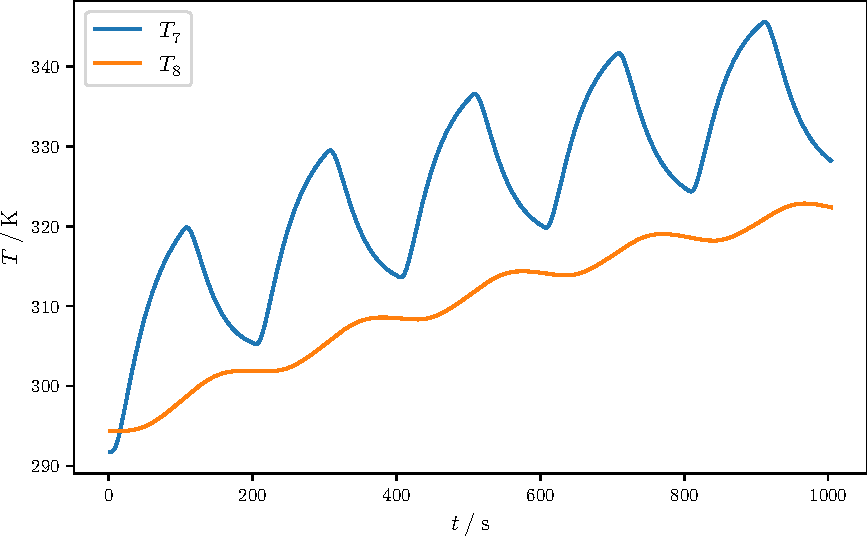
\includegraphics[width = \textwidth]{build/St.pdf}
\end{figure}
\begin{table}
  \centering
  \label{tab:AmplitudeAluminium}
  \caption{Amplituden und Phasendifferenzen des Stahlstabs}
  \sisetup{table-format = 1.2}
  \begin{tabular}{
    S @{${}\pm{}$} S
    S @{${}\pm{}$} S
    S[table-format = 2.2] @{${}\pm{}$} S
    S[table-format = 1.4] @{${}\pm{}$} S[table-format = 1.4]}
     \toprule
     \multicolumn{2}{c}{$A_7 \mathbin{/} \si{\kelvin}$}       &
     \multicolumn{2}{c}{$A_8 \mathbin{/} \si{\kelvin}$}       & 
     \multicolumn{2}{c} {$\symup{\Delta}t_\text{St}  \mathbin{/} \si{\second}$}&
     \multicolumn{2}{c}{$\kappa_\text{St} \mathbin{/} \si{\watt\metre\tothe{-1}\kelvin\tothe{-1}}$}\\
     \cmidrule(lr){1-2} \cmidrule(lr){3-4} \cmidrule(lr){5-6} \cmidrule(lr){7-8}
     \midrule
     7.23 & 0.28 & 0.03 & 0.28 & 80.00 & 0.14 & 3.2818 & 5.5846\\
     7.90 & 0.28 & 0.13 & 0.28 & 72.00 & 0.14 & 4.8696 & 2.5541\\
     7.47 & 0.28 & 0.27 & 0.28 & 56.00 & 0.14 & 7.7447 & 2.4206\\
     8.66 & 0.28 & 0.43 & 0.28 & 60.00 & 0.14 & 7.9928 & 1.7356\\
      \bottomrule
  \end{tabular}
\end{table}
Die Dichte von dem Edelstahl beträgt $\rho_\text{St} = \SI{8000}{\kilogram\per\cubic\metre}$, die spezifische Wärmekapazität 
$c_\text{St} = \SI{400}{\joule\per\kilogram\kelvin}$. Auch der Abstand der beiden Thermoelemente von dem Stahlstab
beträgt $\symup{\Delta} x = \SI{0.03}{\metre}$, so dass sich der Mittelwert der Wärmeleitfähigkeit von
\begin{equation}
  \overline{\kappa}_\text{St} = \SI{6.0(17)}{\watt\per\metre\per\kelvin}
\end{equation}
ergibt. Die hier betrachtete Temperaturwelle wurde mit einer Periodendauer von $\tau = \SI{200.0(1)}{\second}$ erzeugt.
Daraus resultiert eine Frequenz von 
\begin{equation}
  f = \SI{0.0050000(25)}{\per\second} \; \text{.}
\end{equation}
Somit besitzt diese Temperaturwelle eine Wellenlänge von 
\begin{equation}
  \lambda_\text{St} = \SI{0.068(10)}{\metre} \; \text{.}
\end{equation}
Der Fehler der Ampltiuden, des natürlichen Logarithmus des Verhältnis der Amplituden und der Phasendifferenz 
lassen sich mittels der Gaußschen Fehlerfortpfllanzung berechnen:
\begin{align}
  \symup{\Delta} A                                                      &= \sqrt{2} \, \symup{\Delta} T \\
  \symup{\Delta} \left (\symup{\Delta} t \right )                       &= \sqrt{2} \, \symup{\delta} t \\
  \symup{\Delta} \ln \left ( \frac{A_\text{nah}}{A_\text{fern}} \right) &= 
  \sqrt{\frac{1}{A_\text{nah}^2} \left ( \symup{\Delta} A \right )^2 + 
  \frac{A_\text{nah}^2}{A_\text{fern}^4} \left ( \symup{\Delta} A \right ) ^2} 
\end{align}
Die Unsicherheit der Wärmeleitfähigkeit wird ebenfalls mit der Fehlerfortpfllanzung nach Gauß berechnet:
\begin{equation} 
  \symup{\Delta} \kappa = \frac{\rho c \left ( \symup{\Delta} x \right )^2 }
  {2\ln \left ( \frac{A_\text{nah}}{A_\text{fern}} \right ) \symup{\Delta} t} 
  \sqrt{\frac{1}{\left( \symup{\Delta} t\right)^2}
  \left ( \symup{\Delta} \left ( \symup{\Delta} t \right ) \right )^2 + \frac{1}{ \ln \left ( \frac{A_\text{nah}}{A_\text{fern}} \right )^2}
 \left (  \symup{\Delta} \ln \left ( \frac{A_\text{nah}}{A_\text{fern}} \right ) \right )^2}
\end{equation}
Für die Wellenlänge gilt folgende Formel für den Fehler: 
\begin{equation}
 \symup{\Delta} \lambda =  \frac{\sqrt{\frac{2}{\rho c}}} {f} \sqrt{ \frac{\omega}{4 \kappa} \left ( \symup{\Delta} \kappa \right )^2 +
  \frac{\kappa}{4 \omega} \left( \symup{\Delta}\omega\right)^2 +
   4 \frac{\omega\kappa}{f^2} \left(\symup{\Delta} f\right)^2   }
\end{equation}
, wobei
\begin{align}
    \symup{\Delta}f &= \frac{1}{T^2} \symup{\delta} t \\
    \symup{\Delta}\omega &= 2 \symup{\pi} \symup{\Delta} f
\end{align}
gilt. Um die Unsicherheit des Mittelwertes zu erhalten, teilt man die jeweiligen Größen durch die Quadratwurzel der Anzahl der vorhandenen Werte.